\documentclass[11pt]{article}\usepackage{graphicx, color}
%% maxwidth is the original width if it is less than linewidth
%% otherwise use linewidth (to make sure the graphics do not exceed the margin)
\makeatletter
\def\maxwidth{ %
  \ifdim\Gin@nat@width>\linewidth
    \linewidth
  \else
    \Gin@nat@width
  \fi
}
\makeatother

\IfFileExists{upquote.sty}{\usepackage{upquote}}{}
\definecolor{fgcolor}{rgb}{0.2, 0.2, 0.2}
\newcommand{\hlnumber}[1]{\textcolor[rgb]{0,0,0}{#1}}%
\newcommand{\hlfunctioncall}[1]{\textcolor[rgb]{0.501960784313725,0,0.329411764705882}{\textbf{#1}}}%
\newcommand{\hlstring}[1]{\textcolor[rgb]{0.6,0.6,1}{#1}}%
\newcommand{\hlkeyword}[1]{\textcolor[rgb]{0,0,0}{\textbf{#1}}}%
\newcommand{\hlargument}[1]{\textcolor[rgb]{0.690196078431373,0.250980392156863,0.0196078431372549}{#1}}%
\newcommand{\hlcomment}[1]{\textcolor[rgb]{0.180392156862745,0.6,0.341176470588235}{#1}}%
\newcommand{\hlroxygencomment}[1]{\textcolor[rgb]{0.43921568627451,0.47843137254902,0.701960784313725}{#1}}%
\newcommand{\hlformalargs}[1]{\textcolor[rgb]{0.690196078431373,0.250980392156863,0.0196078431372549}{#1}}%
\newcommand{\hleqformalargs}[1]{\textcolor[rgb]{0.690196078431373,0.250980392156863,0.0196078431372549}{#1}}%
\newcommand{\hlassignement}[1]{\textcolor[rgb]{0,0,0}{\textbf{#1}}}%
\newcommand{\hlpackage}[1]{\textcolor[rgb]{0.588235294117647,0.709803921568627,0.145098039215686}{#1}}%
\newcommand{\hlslot}[1]{\textit{#1}}%
\newcommand{\hlsymbol}[1]{\textcolor[rgb]{0,0,0}{#1}}%
\newcommand{\hlprompt}[1]{\textcolor[rgb]{0.2,0.2,0.2}{#1}}%

\usepackage{framed}
\makeatletter
\newenvironment{kframe}{%
 \def\at@end@of@kframe{}%
 \ifinner\ifhmode%
  \def\at@end@of@kframe{\end{minipage}}%
  \begin{minipage}{\columnwidth}%
 \fi\fi%
 \def\FrameCommand##1{\hskip\@totalleftmargin \hskip-\fboxsep
 \colorbox{shadecolor}{##1}\hskip-\fboxsep
     % There is no \\@totalrightmargin, so:
     \hskip-\linewidth \hskip-\@totalleftmargin \hskip\columnwidth}%
 \MakeFramed {\advance\hsize-\width
   \@totalleftmargin\z@ \linewidth\hsize
   \@setminipage}}%
 {\par\unskip\endMakeFramed%
 \at@end@of@kframe}
\makeatother

\definecolor{shadecolor}{rgb}{.97, .97, .97}
\definecolor{messagecolor}{rgb}{0, 0, 0}
\definecolor{warningcolor}{rgb}{1, 0, 1}
\definecolor{errorcolor}{rgb}{1, 0, 0}
\newenvironment{knitrout}{}{} % an empty environment to be redefined in TeX

\usepackage{alltt}

%AMS-TeX packages
\usepackage{amssymb,amsmath,amsthm} 
%geometry (sets margin) and other useful packages
\usepackage[margin=1.25in]{geometry}
\usepackage{graphicx,ctable,booktabs}
\usepackage{color}
\usepackage{listings}
\usepackage{ltablex,calc,enumerate,multirow, float, soul}
\usepackage{hyperref}
\usepackage{longtable, pdflscape}

\begin{document}

\title{(First Draft) A Look at the 2012 Presidential Election}
\author{Eric Hare \& Andee Kaplan}
\date{Nov. 15, 2012}

\maketitle

\section{Introduction}
(1/2 - 1 page)
Motivate your project - why is it exciting? why should people read?
Mention your data source. 
If you go into a topic that a general audience is not familiar with, explain all the NECESSARY parts that allow your audience to understand the work. Don't go excessively beyond the page limit. If you need more than 1/2 page, it's a good sign, that you should switch topics.
Summarize your main finding. 
Outline your data analysis and the structure of the rest of the paper.


\section{Data}
We are primarily working with two data sources to complete our analysis: independent expenditures (PAC) data and polling data. The PAC spending data comes from the \href{http://www.fec.gov/data/IndependentExpenditure.do?format=html&cf=superPAC}{Federal Election Commision} and the polling data comes from \url{http://nationalpolls.com/}. 

\subsection{Variable Definitions}
The variables present in the PAC spending data are defined as follows:
\begin{landscape}
\begin{center}
\begin{longtable}[\textwidth]{l l l p{0.4\textheight} p{0.4\textheight}}
Tag & Field Name	& Data Type	& Description	& Explanation \\
\hline
can\_id  & Candidate ID  & Character &unique ID of candidate for or against whom the expenditure was made	& First character indicates office sought - H=House, S=Senate, P=Presidential. Columns 3-4 are the state abbreviation for Congressional candidates. NOTE - this information is provided by filers and may be missing - in these cases office, state, district and candidate name should appear. \\
spe\_id & Spender ID & Character & Unique ID of committee, individual or group making expenditure	&	Unique FEC ID assigned to the entity submitting reports of independent expenditures \\
spe\_nam & Spender Name &	Character &	Name of committee, individual or group making expenditure	& \\
ele\_typ & Election Type & Character & code for specific election for which expenditure was made & First character indicates election - P=Primary, G=General, S=Special. Next four characters indicate election year. \\
can\_off\_sta & Candidate State	& Character	& Postal state abbreviation for the candidate	& \\	 
can\_off\_dis &	Candidate District & Number &	District number for the candidate	&	District location if spending for/against House candidate.\\
can\_off & Office &	Character &	Office Sought by Candidate &	(H=House, S=Senate, P=President)\\
can\_par\_aff &	Party	& Character &	Party abbreviation for candidate & Dem=Democrat \newline Rep=Republican \\
exp\_amo & Expenditure Amount &	Currency & Dollar amount of specific expenditure & \\
exp\_dat &	Expenditure date &	Date	& Date of specific Expenditure	MM/DD/YYYY & \\	 
agg\_amo & Aggregate amount &	Currency &	Total amount expended during the calendar year, per election, per office sought & \\
sup\_opp &	Support or Oppose &	Character &	S=Support, O=Oppose	& Describes whether the expenditure was made to support or oppose the candidate. \\	 
pur &	Purpose of expenditure &	Character	&	description of the expenditure, e.g. television or radio ad & \\
pay &	name of payee	& Character &	Name of the person or vendor or other entity receiving this payment &\\
file\_num	& Filing number &	Number &	Unique identifier for a submission (which may report several disbursements) & \\
amn\_ind &	Amendment Indicator &	Character &	New report or amendment to a report	& \\	 
tra\_id	& Transaction ID &	Character	& Unique identifier for the transaction (unique within the specific filing	& \\
ima\_num &	Image number &	Number &	Image location for page on which transaction appears & \\
rec\_dt	& Filing receipt date	& Date & Date on which transaction was submitted to FEC	MM/DD/YYYY &\\	 
prev\_file_num & Previous filing number &	Number &	Reference to a filing being amended &	For electronic filings the previous filing number references the filing being amended. For new filings and paper filings this field will be null
\end{longtable}
\end{center}
\end{landscape}
\noindent
The variables present in the polling data are defined as follows:
\begin{center}
\begin{longtable}[\textwidth]{l p{0.15\textwidth} l p{0.3\textwidth}}
Tag & Field Name  & Data Type	& Description\\
\hline
Pollster & Polling Company & Character & Company that conducted the poll. \\
State/US & State & Character & State poll was conducted of. If national poll, then value is ``National".\\
Date & Poll Date & Date & Range of dates that the poll was being conducted.\\
Obama & Support for Mr. Obama & Number & Integer rounded percent of support in the poll. \\
Romney & Support for Mr. Romney & Number & Integer rounded percent of support in the poll.
\end{longtable}
\end{center}
\subsection{Cleaning}
Most of the data cleaning had to be performed on the PAC spending data. We made sure all the columns were formatted correctly in regards to data type (dates are date, numbers are numeric, etc.) before cleaning and reformatting the data more extensively. 

One challenge we faced was that the purpose of independent expenditures column is a free text field on the FEC reporting form. The result was that when trying to explore what PACs spent the majority of their money on, we were unable to group expenditures together. To solve this issue we searched for matches to patterns in the purpose field. We chose these patters by looking at the expenditure purposes and manually finding common threads among the purposes. From these patterns we were able to create buckets that each expense fell in to, as well as high level buckets that more generally classified the expenditures.

An additional complication we faced was with the support/oppose column. This column in conjunction with the candidate column are used to indicate which candidate benefits from the expenditure. An example would be if the support/oppose column is oppose and the candidate name is Romney, then Mr. Obama benefits because the money is being spent to ``oppose Romney". Likewise, if the support/oppose column equals support and the candidate name is Romney, then Mr. Romney benefits.

The polling data did not require very much data cleanup. We needed to split the date range and format the second date as a date for our use. We also removed some differences in state naming by the different pollsters.


\section{Findings}
\begin{knitrout}
\definecolor{shadecolor}{rgb}{0.969, 0.969, 0.969}\color{fgcolor}

{\centering 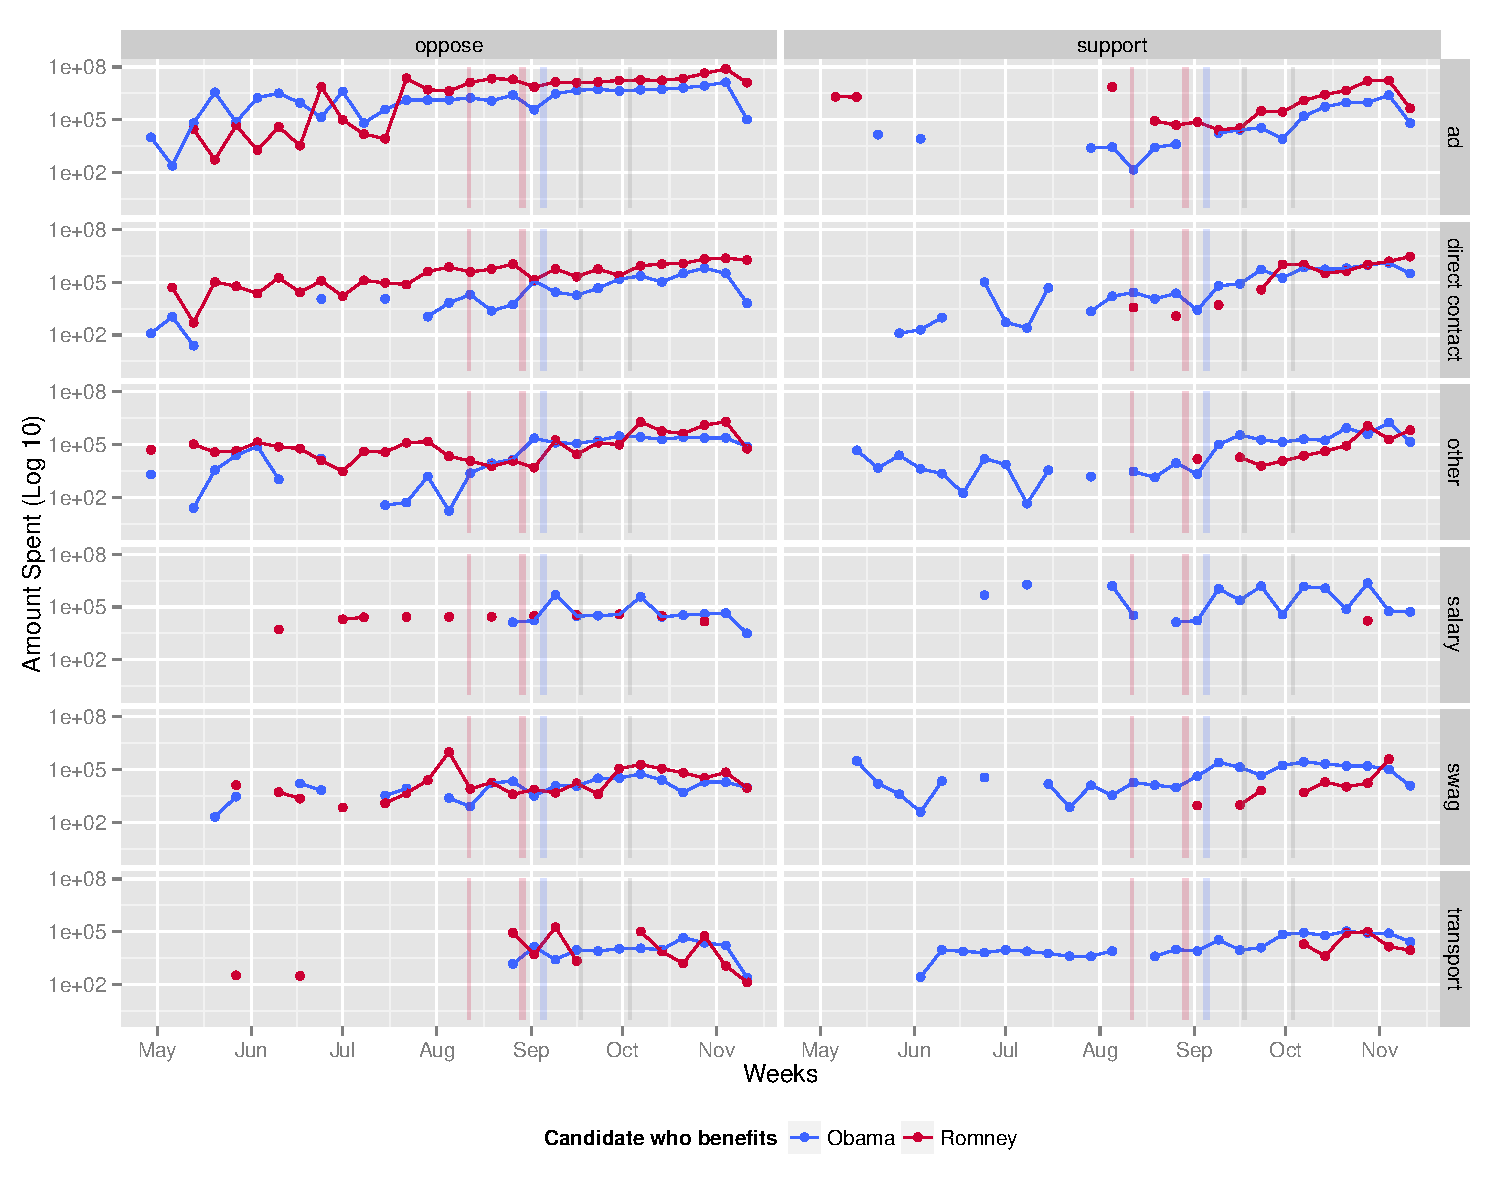
\includegraphics[width=\textwidth]{figure/temporal_plot} 

}


\end{knitrout}



\begin{knitrout}
\definecolor{shadecolor}{rgb}{0.969, 0.969, 0.969}\color{fgcolor}

{\centering 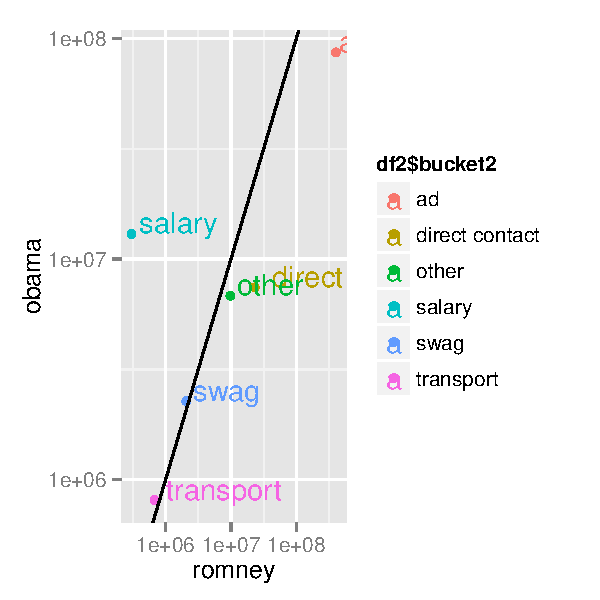
\includegraphics[width=.4\textwidth]{figure/type_plot_11} 

}



{\centering 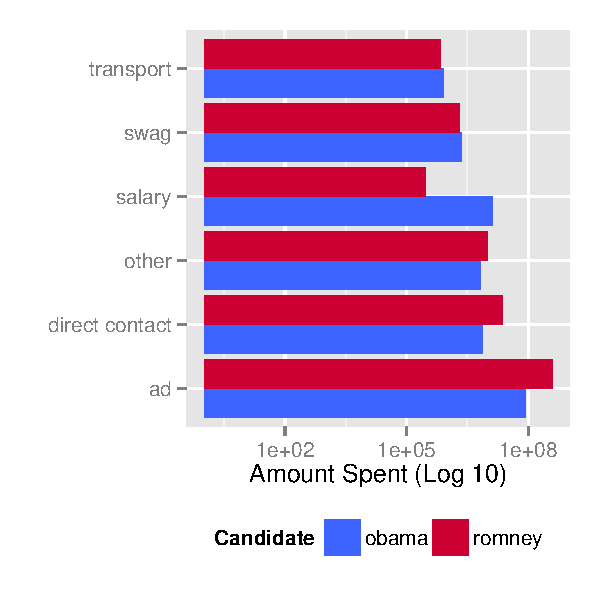
\includegraphics[width=.4\textwidth]{figure/type_plot_12} 

}


\end{knitrout}



\begin{knitrout}
\definecolor{shadecolor}{rgb}{0.969, 0.969, 0.969}\color{fgcolor}

{\centering 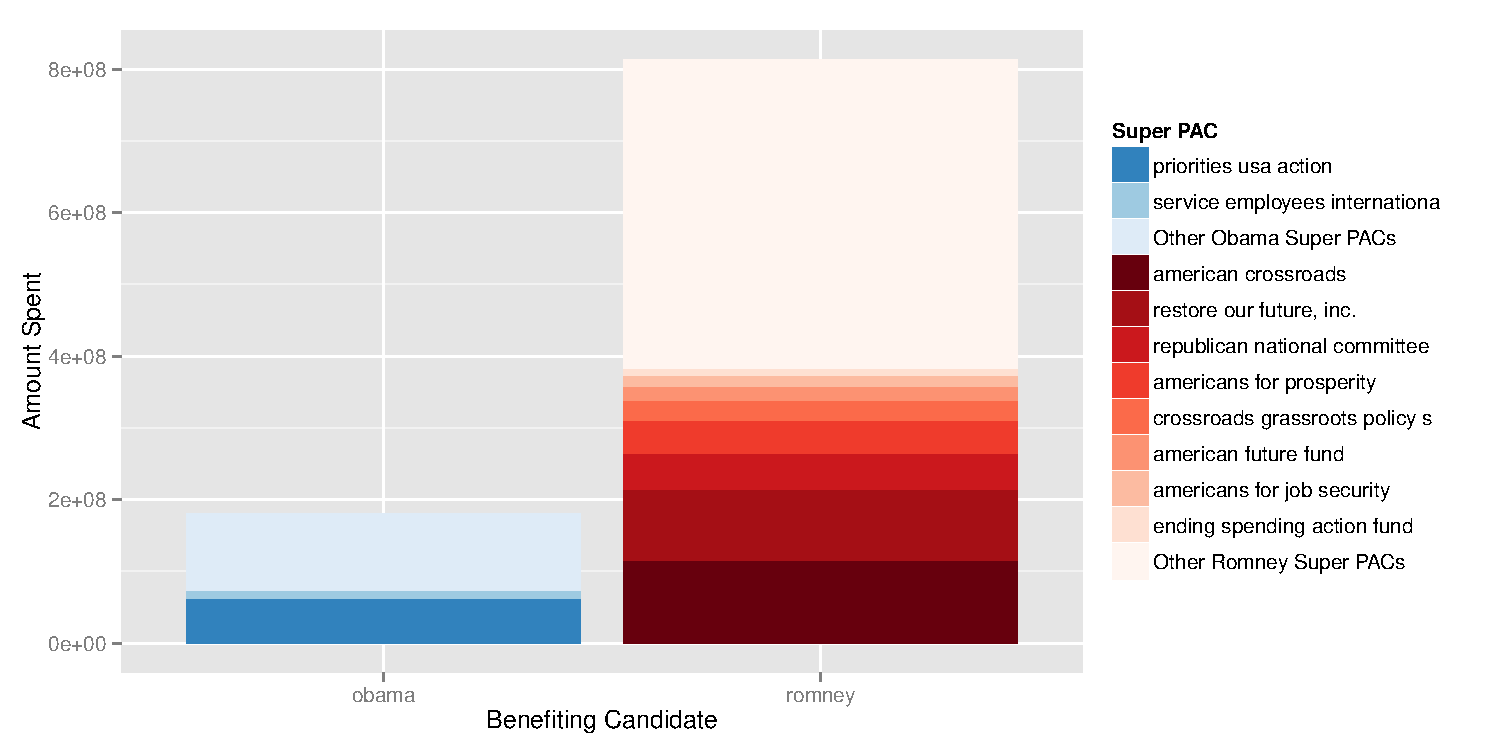
\includegraphics[width=0.5\textwidth]{figure/PAC_plot} 

}


\end{knitrout}


\begin{knitrout}
\definecolor{shadecolor}{rgb}{0.969, 0.969, 0.969}\color{fgcolor}

{\centering 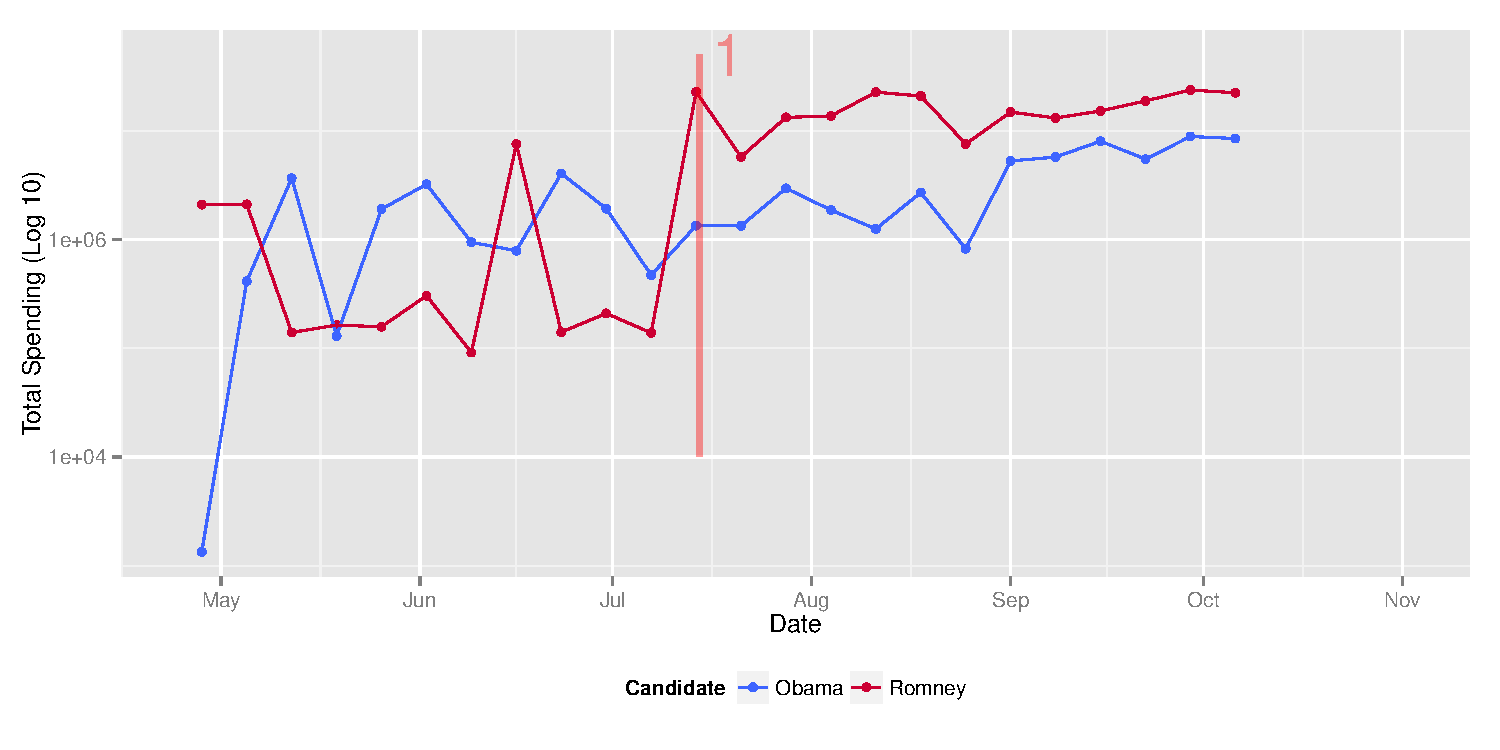
\includegraphics[width=\textwidth]{figure/trend_plot} 

}


\end{knitrout}



\begin{knitrout}
\definecolor{shadecolor}{rgb}{0.969, 0.969, 0.969}\color{fgcolor}\begin{kframe}


{\ttfamily\noindent\itshape\textcolor{messagecolor}{\#\# geom\_smooth: method="auto" and size of largest group is <1000, so using loess. Use 'method = x' to change the smoothing method.}}

{\ttfamily\noindent\itshape\textcolor{messagecolor}{\#\# geom\_smooth: method="auto" and size of largest group is <1000, so using loess. Use 'method = x' to change the smoothing method.}}

{\ttfamily\noindent\itshape\textcolor{messagecolor}{\#\# geom\_smooth: method="auto" and size of largest group is <1000, so using loess. Use 'method = x' to change the smoothing method.}}

{\ttfamily\noindent\itshape\textcolor{messagecolor}{\#\# geom\_smooth: method="auto" and size of largest group is <1000, so using loess. Use 'method = x' to change the smoothing method.}}

{\ttfamily\noindent\itshape\textcolor{messagecolor}{\#\# geom\_smooth: method="auto" and size of largest group is <1000, so using loess. Use 'method = x' to change the smoothing method.}}

{\ttfamily\noindent\itshape\textcolor{messagecolor}{\#\# geom\_smooth: method="auto" and size of largest group is <1000, so using loess. Use 'method = x' to change the smoothing method.}}

{\ttfamily\noindent\itshape\textcolor{messagecolor}{\#\# geom\_smooth: method="auto" and size of largest group is <1000, so using loess. Use 'method = x' to change the smoothing method.}}

{\ttfamily\noindent\itshape\textcolor{messagecolor}{\#\# geom\_smooth: method="auto" and size of largest group is <1000, so using loess. Use 'method = x' to change the smoothing method.}}

{\ttfamily\noindent\itshape\textcolor{messagecolor}{\#\# geom\_smooth: method="auto" and size of largest group is <1000, so using loess. Use 'method = x' to change the smoothing method.}}

{\ttfamily\noindent\itshape\textcolor{messagecolor}{\#\# geom\_smooth: method="auto" and size of largest group is <1000, so using loess. Use 'method = x' to change the smoothing method.}}

{\ttfamily\noindent\itshape\textcolor{messagecolor}{\#\# geom\_smooth: method="auto" and size of largest group is <1000, so using loess. Use 'method = x' to change the smoothing method.}}

{\ttfamily\noindent\itshape\textcolor{messagecolor}{\#\# geom\_smooth: method="auto" and size of largest group is <1000, so using loess. Use 'method = x' to change the smoothing method.}}\end{kframe}

{\centering 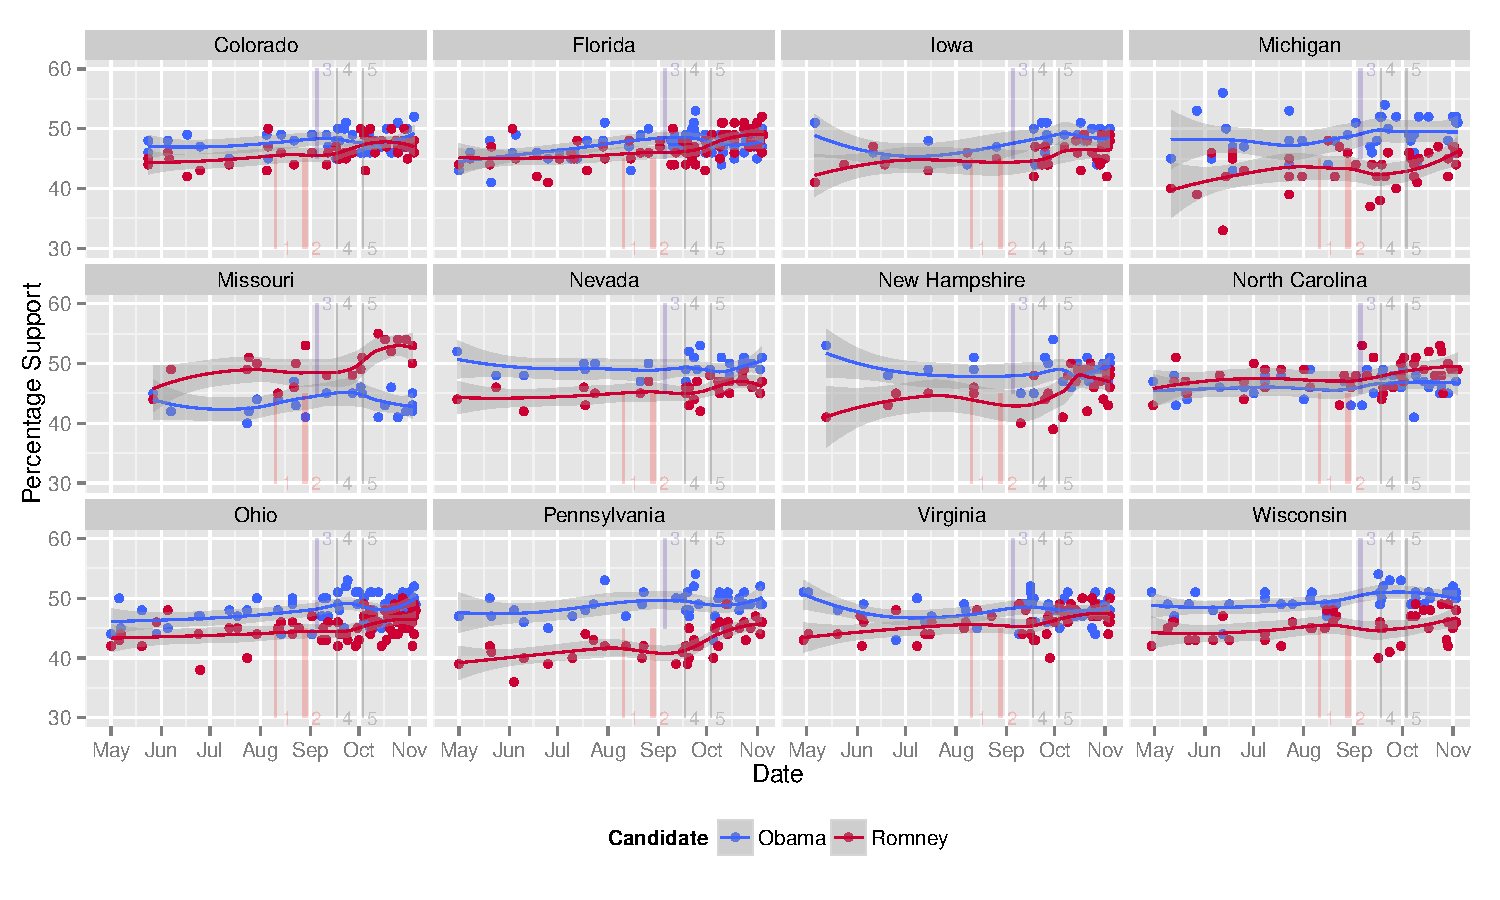
\includegraphics[width=\textwidth]{figure/type_swing_1} 

}


\end{knitrout}


\begin{knitrout}
\definecolor{shadecolor}{rgb}{0.969, 0.969, 0.969}\color{fgcolor}\begin{kframe}


{\ttfamily\noindent\itshape\textcolor{messagecolor}{\#\# geom\_smooth: method="auto" and size of largest group is <1000, so using loess. Use 'method = x' to change the smoothing method.}}\end{kframe}

{\centering 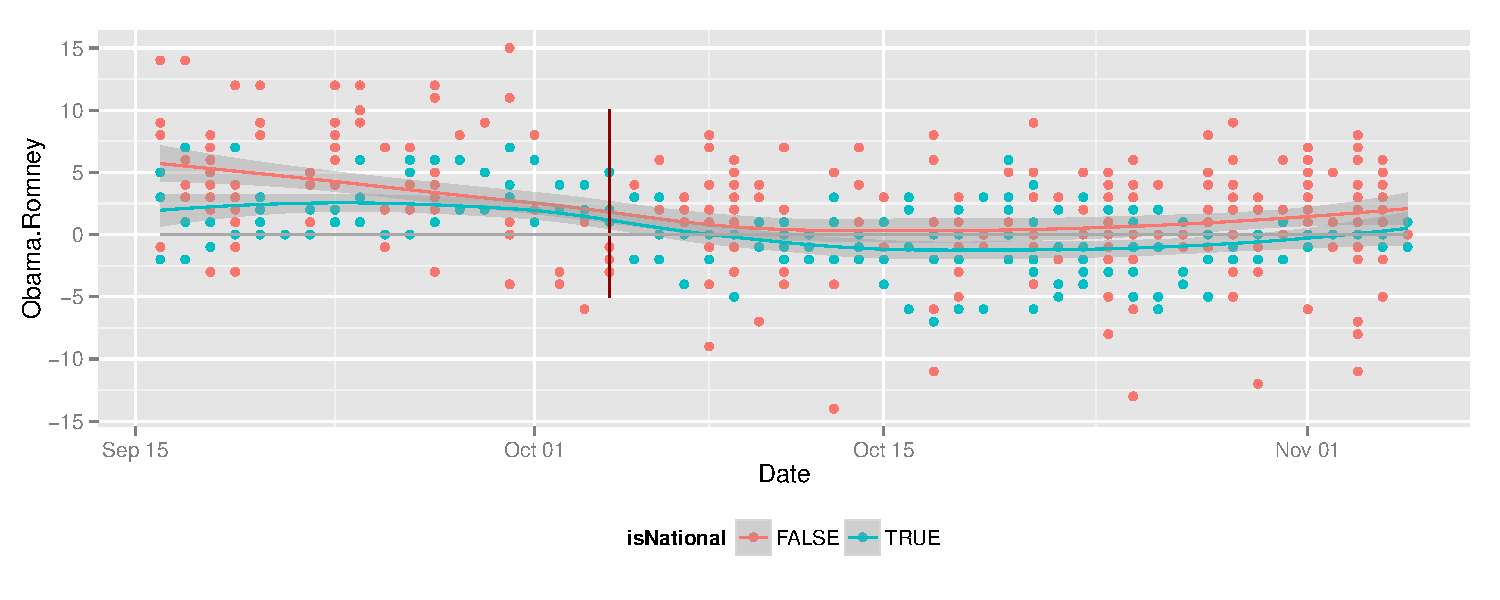
\includegraphics[width=\textwidth]{figure/type_swing_2} 

}


\end{knitrout}



\begin{knitrout}
\definecolor{shadecolor}{rgb}{0.969, 0.969, 0.969}\color{fgcolor}\begin{kframe}


{\ttfamily\noindent\itshape\textcolor{messagecolor}{\#\# geom\_smooth: method="auto" and size of largest group is <1000, so using loess. Use 'method = x' to change the smoothing method.}}\end{kframe}

{\centering 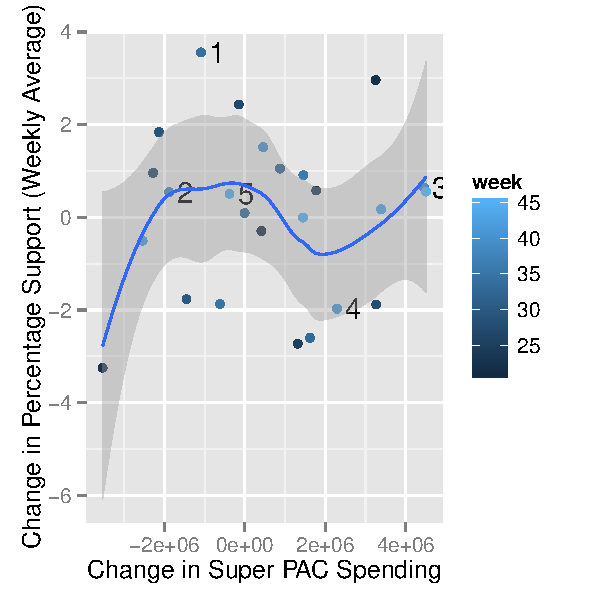
\includegraphics[width=.4\textwidth]{figure/type_support_spend1} 

}

\begin{kframe}

{\ttfamily\noindent\itshape\textcolor{messagecolor}{\#\# geom\_smooth: method="auto" and size of largest group is <1000, so using loess. Use 'method = x' to change the smoothing method.}}\end{kframe}

{\centering 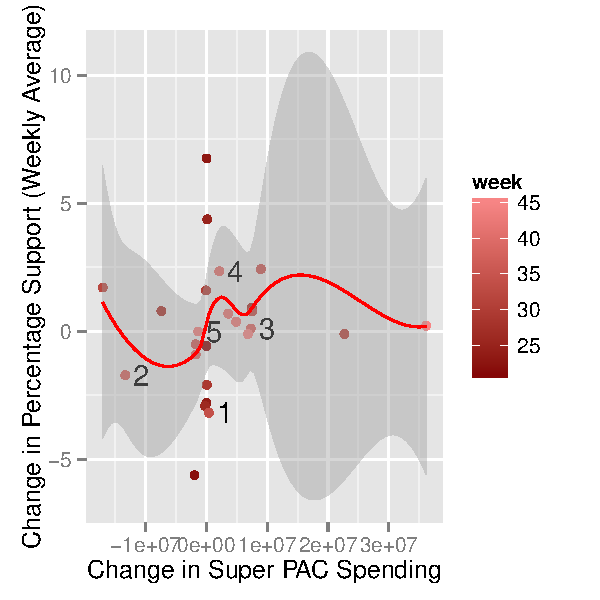
\includegraphics[width=.4\textwidth]{figure/type_support_spend2} 

}


\end{knitrout}


\section{Conclusions/Future Work}
(1/2 page) 
summarize your findings - don't just list them, but try to come up with a cohesive statement. If you started your Intro by posing a question, try to answer it at this point.
For future work come up with at least two good points of how to extend the project or your analysis in a meaningful way.


\end{document}
